\documentclass{standalone}
\usepackage{pgfplots}
\pgfplotsset{compat=newest}

\begin{document}
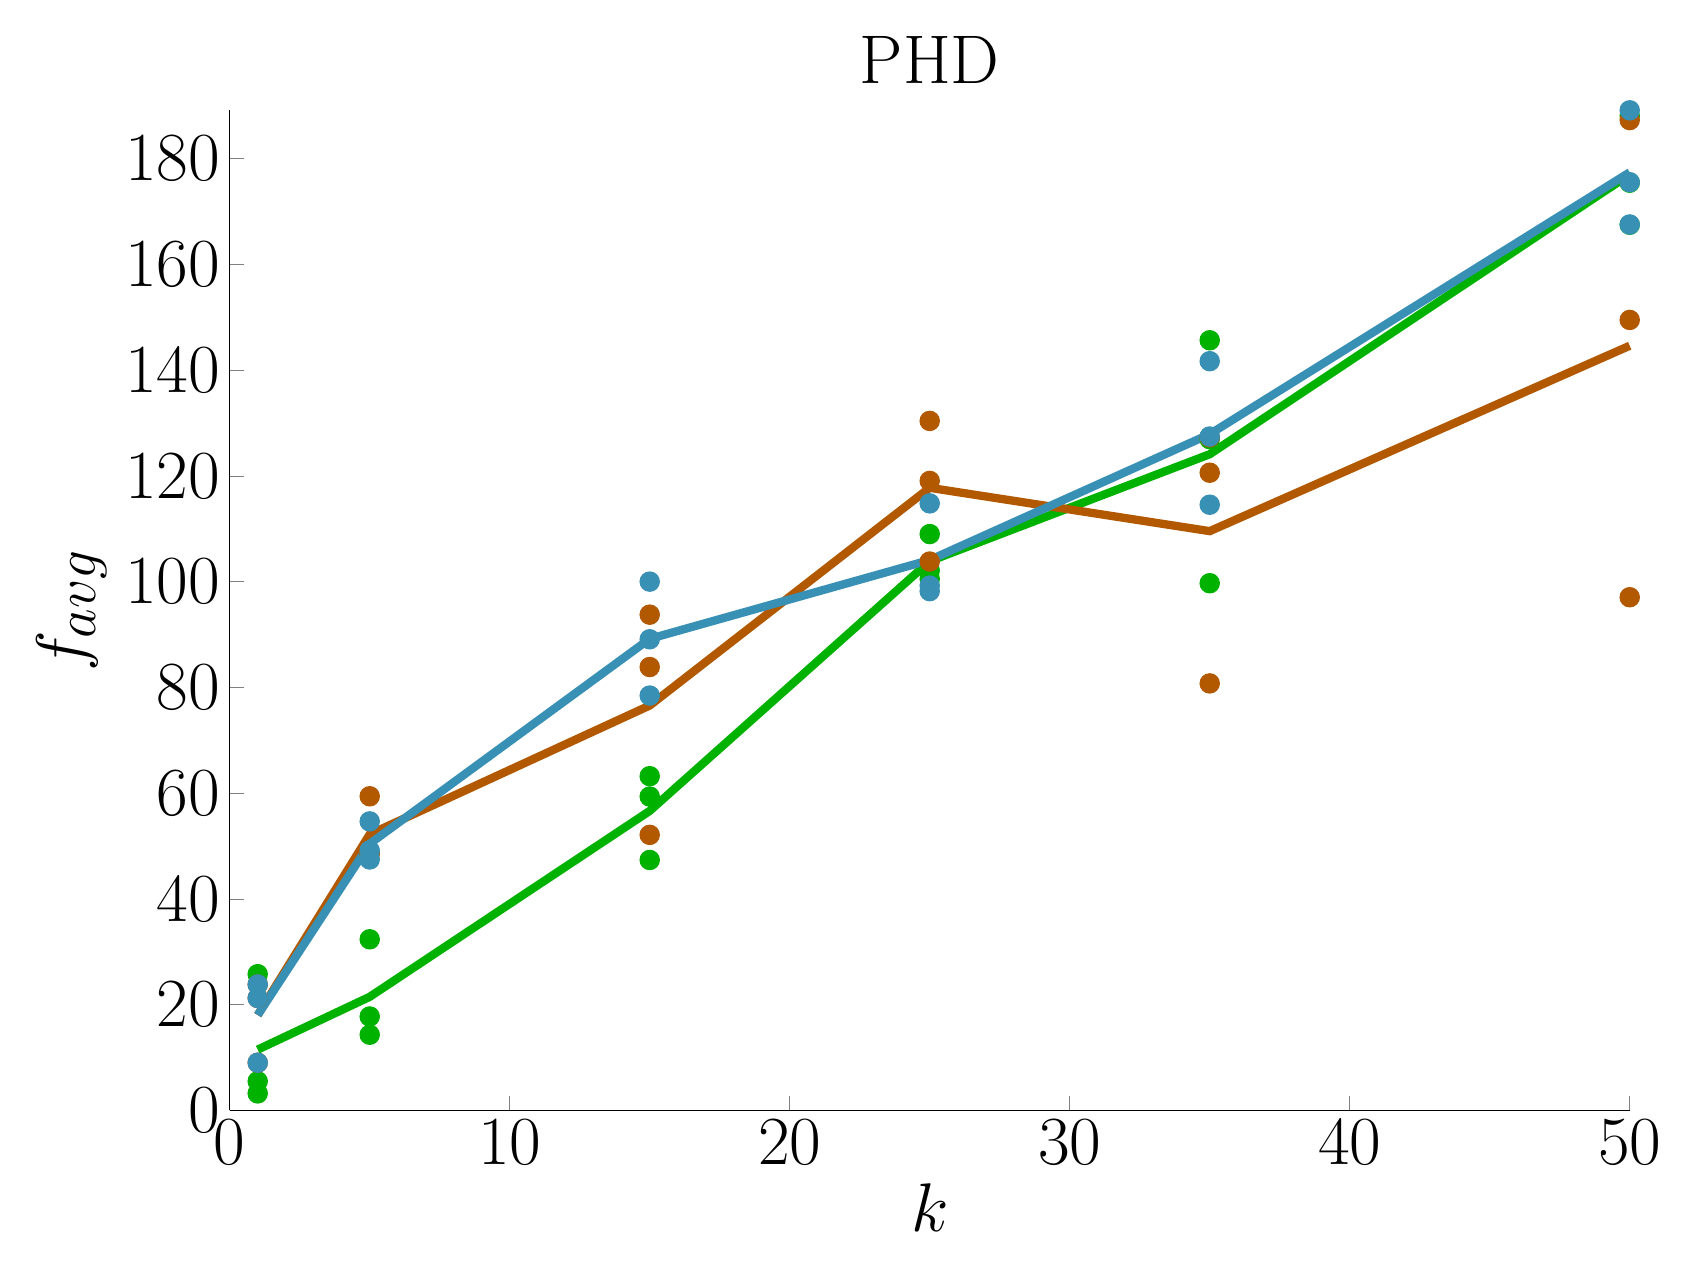
\begin{tikzpicture}

\begin{axis}[%
title style={font=\Huge},
title=PHD,
tick label style={font=\Huge},
label style={font=\Huge},
legend style={font=\Huge},
view={0}{90},
max space between ticks=50pt,
width=7in,
height=5in,
scale only axis,
xmin=0, xmax=50,
xtick={0, 10, 20, 30, 40, 50},
xlabel={$k$},
ymin=0, ymax=189.15,
ylabel={$f_{avg}$},
major tick length=5pt,
axis lines*=left,
legend cell align=left,
clip=false]

\addplot [
only marks,
mark=*,
mark size=3.5pt,
color=green!70!black,
%solid,
%line width=2pt,
]
coordinates{
(1,3.2)(1,5.5)(1,25.75)(5,14.3)(5,17.75)(5,32.35)(15,47.35)(15,59.35)(15,63.2)(25,100.5)(25,102.1)(25,109.0)(35,99.7)(35,126.95)(35,145.65)(50,167.5)(50,175.45)(50,188.1)
};

\addplot [
only marks,
mark=*,
mark size=3.5pt,
color=orange!70!black,
%solid,
%line width=2pt,
]
coordinates{
(1,9.0)(1,21.25)(1,23.8)(5,48.5)(5,48.7)(5,59.4)(15,52.1)(15,83.85)(15,93.75)(25,103.8)(25,119.05)(25,130.4)(35,80.75)(35,120.6)(35,127.3)(50,97.05)(50,149.5)(50,187.3)
};

\addplot [
only marks,
mark=*,
mark size=3.5pt,
color=cyan!70!black,
%solid,
%line width=2pt,
]
coordinates{
(1,9.0)(1,21.25)(1,23.8)(5,47.45)(5,49.15)(5,54.65)(15,78.45)(15,89.1)(15,100.0)(25,98.2)(25,99.25)(25,114.8)(35,114.55)(35,127.45)(35,141.7)(50,167.55)(50,175.55)(50,189.15)
};
p
\addplot [
color=green!70!black,
solid,
line width=3pt
]
coordinates{
(1,11.4833333333)(5,21.4666666667)(15,56.6333333333)(25,103.866666667)(35,124.1)(50,177.016666667)
};

\addplot [
color=orange!70!black,
solid,
line width=3pt
]
coordinates{
(1,18.0166666667)(5,52.2)(15,76.5666666667)(25,117.75)(35,109.55)(50,144.616666667)
};

\addplot [
color=cyan!70!black,
solid,
line width=3pt
]
coordinates{
(1,18.0166666667)(5,50.4166666667)(15,89.1833333333)(25,104.083333333)(35,127.9)(50,177.416666667)
};


\end{axis}
\end{tikzpicture}
\end{document}
